\documentclass[10pt]{article}
\usepackage[letterpaper]{geometry}
\geometry{verbose,tmargin=1in,bmargin=1in,lmargin=1in,rmargin=1in}
\usepackage{setspace}
\usepackage{ragged2e}
\usepackage{color}
\usepackage{titlesec}
\usepackage{graphicx}
\usepackage{float}
\usepackage{mathtools}
\usepackage{amsmath}
\usepackage[font=small,labelfont=bf,labelsep=period]{caption}
\usepackage[english]{babel}
\usepackage{indentfirst}
\usepackage{array}
\usepackage{makecell}
\usepackage[usenames,dvipsnames]{xcolor}
\usepackage{multirow}
\usepackage{tabularx}
\usepackage{arydshln}
\usepackage{caption}
\usepackage{subcaption}
\usepackage{xfrac}
\usepackage{etoolbox}
\usepackage{cite}
\usepackage{url}
\usepackage{dcolumn}
\usepackage{hyperref}
\usepackage{courier}
\usepackage{url}
\usepackage{esvect}
\usepackage{commath}
\usepackage{verbatim} % for block comments
\usepackage{enumitem}
\usepackage{hyperref} % for clickable table of contents
\usepackage{braket}
\usepackage{titlesec}
\usepackage{booktabs}
\usepackage{gensymb}
\usepackage{longtable}
\usepackage{listings}
\usepackage{cancel}
\usepackage{tcolorbox}
\usepackage[mathscr]{euscript}
\lstset{
	basicstyle=\ttfamily\small,
    frame=single,
    language=fortran,
    breaklines=true,
    commentstyle=\color{magenta}\ttfamily,
    postbreak=\raisebox{0ex}[0ex][0ex]{\ensuremath{\color{red}\hookrightarrow\space}}
}

% for circled numbers
\usepackage{tikz}
\newcommand*\circled[1]{\tikz[baseline=(char.base)]{
            \node[shape=circle,draw,inner sep=2pt] (char) {#1};}}

\newcommand{\beq}{\begin{equation}}
\newcommand{\eeq}{\end{equation}}
\newcommand{\beqa}{\begin{equation}\begin{aligned}}
\newcommand{\eeqa}{\end{aligned}\end{equation}}

\titleclass{\subsubsubsection}{straight}[\subsection]

% define new command for triple sub sections
\newcounter{subsubsubsection}[subsubsection]
\renewcommand\thesubsubsubsection{\thesubsubsection.\arabic{subsubsubsection}}
\renewcommand\theparagraph{\thesubsubsubsection.\arabic{paragraph}} % optional; useful if paragraphs are to be numbered

\titleformat{\subsubsubsection}
  {\normalfont\normalsize\bfseries}{\thesubsubsubsection}{1em}{}
\titlespacing*{\subsubsubsection}
{0pt}{3.25ex plus 1ex minus .2ex}{1.5ex plus .2ex}

\makeatletter
\renewcommand\paragraph{\@startsection{paragraph}{5}{\z@}%
  {3.25ex \@plus1ex \@minus.2ex}%
  {-1em}%
  {\normalfont\normalsize\bfseries}}
\renewcommand\subparagraph{\@startsection{subparagraph}{6}{\parindent}%
  {3.25ex \@plus1ex \@minus .2ex}%
  {-1em}%
  {\normalfont\normalsize\bfseries}}
\def\toclevel@subsubsubsection{4}
\def\toclevel@paragraph{5}
\def\toclevel@paragraph{6}
\def\l@subsubsubsection{\@dottedtocline{4}{7em}{4em}}
\def\l@paragraph{\@dottedtocline{5}{10em}{5em}}
\def\l@subparagraph{\@dottedtocline{6}{14em}{6em}}
\makeatother

\newcommand{\volume}{\mathop{\ooalign{\hfil$V$\hfil\cr\kern0.08em--\hfil\cr}}\nolimits}

\setcounter{secnumdepth}{4}
\setcounter{tocdepth}{4}

\title{Schwarz Domain Decomposition of the Heat Equation}
\author{April Novak}


\begin{document}
\maketitle

\section{Introduction}

This final project for CS-267 involves the serial creation and parallelization of a finite element solver to the heat equation, which in its simplest form describes the diffusion of temperature with a heat source:

\beq
\label{eq:eq}
-k\frac{\partial^2 T}{\partial x^2}=\dot{q}
\eeq

where \(k\) is the thermal conductivity, \(T\) the temperature, and \(\dot{q}\) a volumetric heat source. This equation is kept very simple so that the goals of the project can focus entirely on parallelization algorithms, rather than more advanced numerical methods for solving convection-diffusion equations that would be encountered in a class such as MATH-228b (Numerical Solutions of Differential Equations). This equation will be solved using domain decomposition methods in 1-D. 

Due to the second derivative present, two boundary conditions are needed (one on each end of the domain). This presents the fundamental difficulty of parallelizing a domain decomposition  solution to this equation - if the domain is divided amongst different parallel processes or threads, then the equations cannot be solved unless guesses are made for the conditions on the interface boundaries that are created upon domain decomposition. Hence, any parallel solution will require an iterative procedure, where an initial guess for the interior boundary conditions are continually updated by comparing results obtained at domain interfaces. This application is \textit{not} embarrassingly parallel, and if the number of iterations required to reach convergence is very large, then the parallel runtime can easily be longer than the serial runtime. Hence, clever parallel algorithms will be developed such that a net reduction in runtime and good strong and weak scaling are obtained.

The finite element method (FEM) is chosen as the ODE solver because my research focuses on finite element methods applied to Computational Fluid Dynamics (CFD). The remainder of this section will discuss the numerical method applied to the heat equation in 1-D, and some familiarity with numerical methods is assumed so that the brunt of this report can focus on parallelization rather than numerical methods. A large fraction of the discussion of the numerical method is deferred to the Appendix, and only the elements necessary to understand the parallel implementation are discussed here. The FEM is a weighted residual method, that solves the weak form of the governing equation. The weak form is obtained by multiplying Eq. \eqref{eq:eq} by a test function \(\psi(x)\) and integrating over all space:

\beq
\int_{\Omega}\frac{\partial T}{\partial x}k\frac{\partial\psi(x)}{\partial x}dx-\int_{\Gamma}k\frac{\partial T}{\partial x}\psi(x)\cdot\hat{n}dx=\int_{\Omega}\dot{q}\psi(x)dx
\eeq

where \(\Omega\) indicates the entire domain and \(\Gamma\) the boundary of the domain. Now, we assume that the numerical solution \(T_h\) is a sum of coefficients multiplied by expansion functions \(\phi\):

\beq
T_h=\sum_{j=1}^{N}c_j\phi_j(x)
\eeq

where there are \(N\) of these expansion functions defined over the entire domain. Hence, the numerical method reduces to the problem of determining the expansion coefficients \(c_j\) for a user-selected set of \(\phi_j(x)\). The Galerkin FEM specifies that \(\psi\) should come from the same space as \(T_h\). Hence, inserting these expansions into the weak form gives a discrete set of matrix equations that can be solved:

\beq
K_{ij}c_j=R_i
\eeq

where the stiffness matrix is:

\beq
\label{eq:k}
K_{ij}=\int_{\Omega}\frac{\partial \phi_j(x)}{\partial x}k\frac{\partial\phi_i(x)}{\partial x}dx-\int_{\Gamma}k\frac{\partial \phi_j(x)}{\partial x}\phi_i(x)\cdot\hat{n}dx
\eeq

and the load vector is:

\beq
R_{i}=\int_{\Omega}\dot{q}\phi_i(x)dx
\eeq

Additional details relating to this weak formulation necessary for numerical implementation, such as quadrature and local-to-global mappings, are contained in the Appendix. in order to solve this discrete system, as described in the Appendix, it is much easier to solve the system over each element individually and then assemble them together into a single, large, matrix system. A connectivity matrix is used to describe how the local element nodes map into the global system. The formation of this connectivity matrix is also deferred to the Appendix. 

The important feature of this connectivity matrix from the perspective of parallelization is that the structure of the sparse stiffness matrix is all held in the structure of the connectivity matrix. The global stiffness matrix can only be formed by looping through the columns of the connectivity matrix. There is not a one-to-one correspondence of entries in local matrices to entries in global matrices. That is, some entries overlap due to continuity requirements at inter-element nodes. Because the stiffness matrix is sparse, the Compressed Sparse Row (CSR) format was implemented in my code to reduce the storage requirements from roughly \(N^2\) to \(N\). This is described in Section \ref{sec:CSR}. The application of boundary conditions is rather simple, and is described in the Appendix.

Once these boundary conditions have been incorporated into the matrix system, the matrix system can be solved by your favorite linear algebra routine. For this assignment, the Conjugate Gradient (CG) method is selected to solve this symmetric system because this will provide more flexibility for exploring parallelization algorithms than simply using some routine from BLAS or LAPACK. To solve a matrix system \(\textbf{K}a=R\) by the CG method requires rewriting the governing equation as the minimization of a potential \(\Pi\). The exact solution is obtained by taking the gradient of this potential with respect to each of the expansion coefficients in the vector \(a\), and setting that gradient equal to zero. The minimizer to the potential \(\Pi\) is also a solution to the matrix system. Krylov methods are a class of methods that successively update an initial iterate guess in ways that minimize \(\Pi\) with each iteration. Details of the CG method are deferred to the Appendix.

Given an initial guess for the solution \(a\), CG iterations are performed until there is acceptably small difference between two successive iterates \(a^i\) and \(a^{i+1}\). This numerical method is selected due to its relative simplicity. This concludes the theoretical discussion of the FEM applied to this simple 1-D heat equation. The next section discusses steps taken to obtain a fast serial implementation of this algorithm, and will go into more detail regarding exactly how this method can be implemented in code.

\section{Serial Implementation}

This section discusses the serial code that is used as a launching point for parallel algorithms. As a nuclear engineering student interested in computational methods, you will quickly learn that the consequences of errors in codes used to design nuclear reactors can potentially be very high. Hence, in this field there is very slow acceptance of new modeling codes since each new code must undergo rigorous verification and validation. {\it Many} nuclear simulation codes are written in Fortran, so I used this project as an opportunity to learn how to program in Fortran 2003. The code is written in a modular format. Psuedo-code for the overall program structure is as follows:

\begin{lstlisting}
! read in problem parameters from command line and namelist
call read_namelist()
call read_commandline()

! initialize problem variables based on user inputs
call initialize_global_mesh()
call define_quadset()
call define_shapefunctions()

! determine elemental matrices
call elementalload()
call elementalstiffness()

! find a good initial guess to serve as input to the CG solver
! ...... discussed later ....... !

! form location matrix
LMfine = locationmatrix(global%n_el, global%n_nodes)

! form global load vector and apply boundary conditions
global%rglob  = globalvector(LMfine, rel, global%n_nodes)

! determine CSR storage of global stiffness matrix
call form_csr(LMfine, global%n_nodes, rows)

! call CG method to solve
solution = conjugategradient(rows, guess, global%rglob, global%BCs)
\end{lstlisting}

So, every problem begins by initializing problem variables and determining the elemental matrices. An initial guess is required for the CG solver, and can be as naive as a vector of zeros, or determined in a more fancy way. Then, the global load vector is determined by looping through the connectivity matrix and the CSR storage of the stiffness matrix determined. Finally, the CG method is called with the initial guess and the {\tt rows} data structure holding the CSR information. The remainder of this section will discuss efforts made in the serial code to achieve better performance.

\subsection{CSR Format}
The most important improvement above the first naive code (not discussed in this report) is the storage of the global stiffness matrix in CSR form. The global stiffness matrix is sparse. With linear elements in 1-D, a maximum of \(4N\) nonzero elements would need to be stored (with \(N\) the number of elements). Hence, the memory improvement associated with implementing CSR storage offers about \(\mathscr{O}(N)\) less storage requirements. The difficulty with implementing CSR storage here is that the structure of the matrix is not known until every column of the connectivity matrix is looped over. The only way to form the CSR for this application was to determine a relationship between the number of times a node number appears in the connectivity matrix with how many nonzero entries appear on that row in the global matrix. This relationship is different depending on if the mesh is 1-D, 2-D, or 3-D, and on the type of element (2-D triangles vs. 2-D squares), but for 1-D elements, if a node number appears \(n\) times in the connectivity matrix, then that row in the global matrix has \(2(n-1)\) nonzero entries. The CSR storage is formed by looping over the location matrix and counting the number of times each node number appears, and then saving the nonzero values in a vector and the column numbers (which are determined as the entries of the location matrix for that element) in a vector. The realization that the entries don't need to be stored in ascending column order (as CSR storage is discussed in the slides) makes reorganization of the data unnecessary, and hence this algorithm provides a great reduction in memory requirements. 

\subsection{Vectorization}

Single Instruction, Multiple Data (SIMD) is the process by which a single instruction is used to perform an operation on multiple pieces of data at the same time. When instructed with the appropriate vectorization flags, the compiler will try to find SIMD parallelism and use them as much as possible. Using the GNU compiler, automatic vectorization can be attempted using the {\tt -O3} flag. Using this flag, as opposed to zero compiler flags, yields a dramatic performance improvement. The great benefit of the CSR storage is not fully appreciated without an understanding of why some loops cannot be automatically vectorized. The naive formation of the global stiffness matrix leads to loop-dependence because values can overlap in any particular entry \(K(i, j)\):

\begin{lstlisting}
do k = 1, number_of_elements
  do i = 1, number_element_nodes
    do j = 1, number_element_nodes
      ! loops cannot be vectorized here
      K(LM(i, k), LM(j, k)) = K(LM(i, k), LM(j, k)) + k_local(i, j)
    end do
  end do
end do
\end{lstlisting}

Likewise, without the CSR storage, 



However, compilers in general cannot vectorize code to the full extent possible, so some manual modifications were investigated to see if they could improve performance. 





The Intel compiler provides good vectorization reports when using the {\tt -qopt-report=3} compiler option. 

\section{Parallel Implementation}
This section discusses parallelization of the serial code developed in the previous section. In general, there are two very different parallelization strategies here - the first involves domain decomposition amongst parallel threads, where each parallel thread then runs a complete FEM solution, with iteration between threads until all threads agree on the values of the solution at the boundaries between the spatial domain allocated to each process. Alternatively, a single FEM problem can be run (with no need to iterate boundary conditions because the domain is not decomposed), and the work for the single FEM solve distributed amongst parallel instances. Domain decomposition is more often used in large applications in practice because the domain may be so large and the problem information (such as discretized material properties, multiple components of solution vectors, etc.) so large that it cannot fit into the memory of a single processor. So, domain decomposition is pursued for this project, with the possibility of using OpenMP within an MPI process to obtain enhanced performance.

The basic domain decomposition algorithm is shown below for a 1-D domain. Each parallel process solves a subregion of the domain, where the union of all of the subregions equals the original domain. To perform this step, boundary conditions must be imposed on all edges of the domain allocated to each process (since the Poisson equation has two derivatives). All locations where boundary conditions are imposed are indicated with vertical red lines. Because the solution is not known a-priori, the boundary conditions on the interior of the domain, between adjacent domains, must be guessed. After each process solves its subregion, there are two possible algorithms for solving the interface problem. First, all of the processes can communicate the values they compute for solutions one element on each side of the domain interfaces to a single process. This process would then solve the interface problem to determine updated guesses for the domain-interface values, and the entire iterative process repeated. This is the procedure that must be used in higher dimensions for unstructured meshes, since the interface problems would not necessarily be decouple as they are in 1-D. The second approach, which can {\it only} be used in the interface problems are decoupled from each other, is for the process to the left of each interface problem to communicate their boundary value to the processor to the right, and then that process solve a single interface problem. This reduces the number of broadcast operations required and also has the potential to reduce overall runtime because 1) each processor at most communicates with two other processors, and 2) a single process does not need to wait for all processes to finish their domain computations. Again, this is only possible if the interface problems are fully decoupled, which is the case for 1-D.

\begin{figure}[H]
\centering
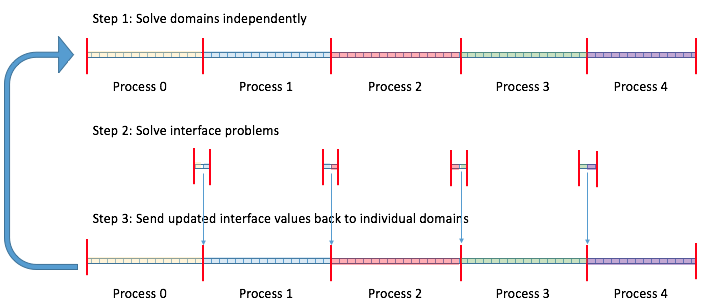
\includegraphics[width=0.8\textwidth]{../figures/1D-dd.png}
\caption{Basic algorithm for 1-D domain decomposition.}
\end{figure}

Because it is easier to implement, the first version of this algorithm is implemented such that the rank 0 process solves the interface problem. The high-level pseudo code for this algorithm is as follows. For a single iteration, all processors solve their domains, and then a barrier is required to ensure that they have all completed before broadcasting their boundary values to the rank 0 process. Once the rank 0 process has received all of the boundary information, it solves the {\tt numprocs - 1} interface problems, and updates the domain-domain boundary conditions stored in memory. Then, the rank 0 process broadcasts these updated boundary conditions to all processes. In order to determine if the looping should continue, a reduction operation is performed to collect the relative change in the domain-domain boundary conditions.

\begin{lstlisting}
do while (iteration_error > tol)
	! each processor solves for its domain

	call mpi_barrier(mpi_comm_world, ierr)
	call mpi_gatherv(local_bcs, mpi_real8, interface_bcs, 2, 2, mpi_real8, 0, mpi_comm_world, ierr)
	
	! rank 0 process solves the interface problems
	if (rank == 0) then
		do interface = 1, numprocs - 1
			! solve interface problem
			! update matrix of BCs
		end do
	end if
	
	call mpi_bcast(local_bcs, numprocs * 2, mpi_real8, mpi_comm_world, ierr)
	
	! determine iteration_error
	call mpi_allreduce(abs(local_bs(1, rank) - previous_bcs(1, rank)), iteration_error, 1, mpi_real8, mpi_comm_world, ierr)
end do
\end{lstlisting}


\section{Appendix}
\subsection{Details of the Finite Element Method}
This section contains additional discussion of the FEM that is necessary to fully understand the code developed, but not necessary to appreciate parallelization algorithms.

\subsubsection{The Element-Wise Weak Form}
The stiffness matrix shown in Eq. \eqref{eq:Stiffness} consists of the multiplication of the derivatives of \(\phi_i(x)\) with \(\phi_j(x)\). If these shape functions are defined over the {\tt entire} domain, then the stiffness matrix will be a dense matrix. On the other hand, if we choose these shape functions to be nonzero only over a single small region of the domain, then the product of cross terms will be zero for most of the matrix, since the effect of a single shape function will be very localized. This will produce sparse matrices, which will be much easier to work with and will also permit easier extension as a numerical method over a discretized domain. Hence, the expansion for the solution and test function for a {\it single} element (``element'' is used in this sense as a small region of the domain, i.e. a meshing software would divide up a continuous domain into discrete elements) becomes:

\beq
T_h^e=\sum_{j=1}^{n_{en}}c_j^e\phi_j^e(x)
\eeq

where the \(e\) superscript indicates the element and \(n_{en}\) are the number of element nodes. A nodal basis is selected for the shape functions. This means that, over a single element, the shape functions are unity at their corresponding node, and zero at the other nodes. The matrix equation \(K_{ij}c_j=R_i\) can be written for written for each individual element, with a post-processing step that takes the system of equations for each element and connects them all together to enforce solution continuity at element interfaces. 

\beq
K_{ij}^ec_j^e=R_i^e
\eeq

where

\beq
K_{ij}^e=\int_{\Omega^e}\frac{\partial \phi_j(x)}{\partial x}k\frac{\partial\phi_i(x)}{\partial x}dx-\int_{\Gamma^e}k\frac{\partial \phi_j(x)}{\partial x}\phi_i(x)\cdot\hat{n}dx
\eeq

\beq
R_{i}^e=\int_{\Omega^e}\dot{q}\phi_i(x)dx
\eeq

such that the domain of integration is only over a single element. However, the system of equations for each element, \(K_{ij}^ec_j^e=R_i^e\), is singular, and cannot be solved independently of the other elements, since we require solution continuity at inter-element nodes. This requires the formation of a connectivity matrix.

\subsubsection{The Connectivity (Location) Matrix}
Figure \ref{fig:FEmesh} shows a simple FE mesh, where the numbers illustrate the global node numbering. A mapping is required from the elemental perspective to this global mesh. The location matrix contains this information - each column of the location matrix gives the global node numbers that correspond to the local node numbers. The local nodes must always be numbered in a consistent manner (i.e. always clockwise or always counterclockwise) so that the Jacobian of the local to global transformation is positive. The first five columns of the location matrix for this mesh, for illustration, would be:

\beq
\label{eq:LM}
LM=\begin{bmatrix}
1 & 2 & 3 & 4 & 5 & \cdots\\
2 & 3 & 4 & 5 & 6 & \cdots\\
11 & 12 & 13 & 14 & 15 & \cdots\\
10 & 11 & 12 & 13 & 14 & \cdots\\
\end{bmatrix}
\eeq

where the nodes have been numbered counterclockwise.

\begin{figure}[H]
\centering
\includegraphics[width=0.8\textwidth]{../figures/FEmesh.pdf}
\caption{Global node numbering in a simple FE mesh. Source:\newline {\tt http://opensees.berkeley.edu/wiki/index.php/}\newline{\tt Simply\_supported\_beam\_modeled\_with\_two\_dimensional\_solid\_elements}}
\label{fig:FEmesh}
\end{figure}

For structured meshed, this location matrix is fairly easy to determine, but for unstructured meshes where there is not necessarily a pattern to the node connectivity, would be provided by a meshing software such as Cubit.  Once this location matrix is known, the elemental systems of equations \(K_{ij}^ec_j^e=R_i^e\) can be assembled into the global system of equations \(K_{ij}c_j=R_i\). The fundamental reason why it is preferred to assemble the equations for each element individually, and {\tt then} assemble these into a global system, is that we have chosen shape functions that are only nonzero over an element and its immediate neighbors. This algorithm is inherently local until we get to the step requiring continuity, and it is hence natural to avoid unnecessary computations of zero integrals by only computing the integrals over each element, and then assembling these systems together at the end right before the numerical solve. For better illustration, several entries of \textbf{K} are assembled as follows for the location matrix given in Eq. \eqref{eq:LM}.

\beqa
K(1, 1) =& k(1, 1)^{e=1}\\
K(1, 2) =& k(1, 2)^{e=1}\\
K(2, 2) =& k(2, 2)^{e=1}+k(1, 1)^{e=2}\\
K(2, 11) =& k(2, 3)^{e=1}\\
K(12, 12) =& k(3, 3)^{e=2}+k(4, 4)^{e=3}\\
\eeqa

where a new notation of lowercase \(k\) representing \(K^e\) is used.

\subsubsection{Boundary Conditions}
Once the global matrix has been assembled, any Dirichlet boundary conditions must be applied (Neumann boundary conditions have naturally been applied by the form of the perimeter integral in Eq. \eqref{eq:k}). Dirichlet boundary conditions are strictly imposed by removing the Dirichlet nodes from the global matrix system. For a 1-D domain consisting of four linear elements (two nodes per element), the global matrix system \(\textbf{K}c=\textbf{R}\) before imposition of Dirichlet boundary conditions is:

\beq
\textbf{K}=
\begin{bmatrix}
k(1, 1)^{e=1} & k(1, 2)^{e=1} & 0 & 0 & 0\\
k(2, 1)^{e=1} & k(2, 2)^{e=1}+k(1, 1)^{e=2} & k(1, 2)^{e=2} & 0 & 0\\
0 & k(2, 1)^{e=2} & k(2, 2)^{e=2}+k(1, 1)^{e=3} & k(1, 2)^{e=3} & 0\\
0 & 0 & k(2, 1)^{e=3} & k(2, 2)^{e=3}+k(1, 1)^{e=4} & k(1, 2)^{e=4}\\
0 & 0 & 0 & k(2, 1)^{e=4} & k(2, 2)^{e=4}\\
\end{bmatrix}
\eeq

\beq
\textbf{R}=\begin{bmatrix}
R_1^{e=1} \\ R_2^{e=1}+R_1^{e=2}\\R_2^{e=2}+R_1^{e=3}\\R_2^{e=3}+R_1^{e=4}\\R_2^{e=4}\\
\end{bmatrix}
\eeq

To apply Dirichlet boundary conditions at nodes \(1\) and \(5\), the off-diagonal terms in the stiffness matrix are set to zero and the corresponding terms in the global load vector are set to the Dirichlet values. For instance, to impose Dirichlet conditions of \(T(node 1)=3.5\) and \(T(node 5) = 10.5\), the global matrix system becomes:

\beq
\textbf{K}=
\begin{bmatrix}
1 & 0 & 0 & 0 & 0\\
k(2, 1)^{e=1} & k(2, 2)^{e=1}+k(1, 1)^{e=2} & k(1, 2)^{e=2} & 0 & 0\\
0 & k(2, 1)^{e=2} & k(2, 2)^{e=2}+k(1, 1)^{e=3} & k(1, 2)^{e=3} & 0\\
0 & 0 & k(2, 1)^{e=3} & k(2, 2)^{e=3}+k(1, 1)^{e=4} & k(1, 2)^{e=4}\\
0 & 0 & 0 & 0 & 1\\
\end{bmatrix}
\eeq

\beq
\textbf{R}=\begin{bmatrix}
3.5\\ R_2^{e=1}+R_1^{e=2}\\R_2^{e=2}+R_1^{e=3}\\R_2^{e=3}+R_1^{e=4}\\10.5\\
\end{bmatrix}
\eeq

\section{The Conjugate Gradient Method}
The CG method requires computation of the residual:

\beq
r^i=R-\textbf{K}a^i
\eeq

where \(i\) is the iteration index.Each update to the solution iterates is performed according to:

\beq
\label{eq:CGUpdate}
a^{i+1}=a^i+\lambda^iz^i
\eeq

where the update scales by \(z^i\):

\beq
\label{eq:ZUpdateCG}
z^i=r^i+\theta^iz^{i-1}
\eeq

where \(\theta^i\) is a parameter chosen such that \(z^i\) is \(\textbf{K}\)-conjugate to \(z^{i-1}\), or:

\beq
\label{eq:kconjugate}
z^{T,i}\textbf{K}z^{i-1}=0
\eeq

In other words, the search direction is a combination of a move in the reverse direction of the gradient (method of steepest descent) plus a motion perpendicular to that direction. This helps to avoid duplicate searching in the same general area. For the very first iteration, it is common to select \(z^1=r^1\). Simply plugging in Eq. \eqref{eq:ZUpdateCG} to Eq. \eqref{eq:kconjugate} gives:

\beq
\theta^i=-\frac{r^{T,i}\textbf{K}z^{i-1}}{z^{T,i-1}\textbf{K}z^{i-1}}
\eeq

Plugging in Eq. \eqref{eq:CGUpdate} into Eq. \eqref{eq:IterativeMethodsPotential} and then taking the partial derivative with respect to \(\lambda^i\), the optimal \(\lambda^i\) is:

\beq
\label{eq:UpdateCG}
\lambda^i=\frac{z^{T,i}r^i}{z^{T,i}\textbf{K}z^i}
\eeq

\end{document}
